\section{Steering Controller}\label{sec:steeringController}
The steering controller is being split up in two controllers. One to control the angular movement of the vehicle, with the use of the servo and magnetometer, so the car can follow the right direction and another controller to keep the vehicle on the route, using the GoT system. Both controller will be design out from the steering model from \secref{sec:SteeringModel}. 

A problem, that have occur, is that the magnetometer do not work inside, which makes testing with both the GoT system and magnetometer together impossible, as the GoT system is located indoor. This problem effects the testing of some parts of the system, which will only be simulated.

As the angular controller works on the first part of the plant, it will be design first.

\subsection{Directional controller}
The purpose of the directional controller is to have the vehicle turn according to a reference, which the controller receives from the route control, see \secref{Finalprototype}. The design will start out with a proportional controller for the directional controller.
%
\subsubsection{Proportional controller}
A proportional controller implemented in the directional model, see \secref{sec:SteeringModel}, can be seen in \figref{fig:PconAngpic}.
%
\begin{figure}[H]
  \centering
  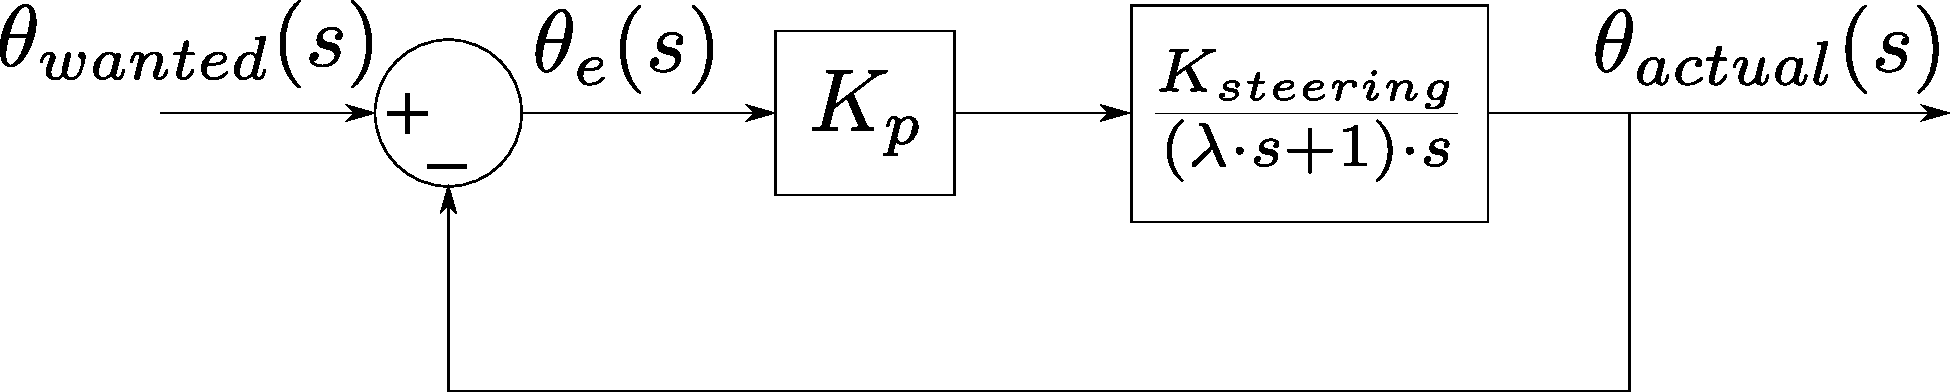
\includegraphics[scale=0.7]{figures/angularController.pdf}
  \caption{Illustration of a proportional controller for the directional steering.}
  \label{fig:PconAngpic}
\end{figure}\vspace{-5mm}
%
This will yield the following closed loop transfer function:
%
\begin{flalign}
  \eq{ \frac{\theta_{actual}}{\theta_{wanted}} }{ \frac{\frac{ K_p \cdot K_v \cdot K_s }{ (\lambda \cdot s + 1) \cdot s } }{ \frac{ K_p \cdot K_v \cdot K_s }{ (\lambda \cdot s + 1) \cdot s } + 1} }&\label{eq:PconAng}
\end{flalign}
%
According to \appref{app:steeringGainTest}, the values of $K_s$ and $K_v$ are not needed independently. they are therefore combined to the steering gain, \si{K_{steering}}. From \appref{app:steeringGainTest}, the steering gain can be calculated, with \eqref{eq:PconAng10}.
%
\begin{flalign}
\eq{K_{steering}}{0,3 \cdot v - 0,034}
\label{eq:PconAng10}
\end{flalign}
%
As $v$ is the wanted velocity, which is 1,4 $m \cdot s^{-1}$, $K_{steering}$ is equal to 0,386. And with lambda equal to the servo duty cycle time constant on 30 ms \secref{Servo}, the transfer function yields:
%
\begin{flalign}
  \eq{ \frac{\theta_{actual}}{\theta_{wanted}} }{ \frac{\frac{ K_p \cdot 0,386 }{ (0,03 \cdot s + 1) \cdot s } }{ \frac{ K_p \cdot 0,386 }{ (0,03 \cdot s + 1) \cdot s } + 1} \Rightarrow \frac{1}{\frac{ 0,03 \cdot s^2 + s }{ K_p \cdot 0,386 } + 1}  }&\label{eq:PconAng2}
\end{flalign}
%
From the test done in \appref{app:LinearAreaKp}, it is know, that the steering gain is not constant for different $K_p$ values. The test illustrates a linear area occurs between a $K_p$ value of 1,5 and 3, where the steering gain is constant if the velocity is kept the same. From \eqref{eq:PconAng2}, it can be seen that the time constant will decrease, if the $K_p$ increases. To get the fastest reacting system, with this limitation, $K_p$ is set to be 3. This give a transfer function which yields:
%
\begin{flalign}
  \eq{ \frac{\theta_{actual}}{\theta_{wanted}} }{ \frac{1}{\frac{ 0,03 \cdot s^2 + s }{ 3 \cdot 0,386 } + 1} \Rightarrow \frac{1}{ 0,026 \cdot s^2 + 0,86 \cdot s + 1} }&\label{eq:PconAng4}
\end{flalign}
%
From this transfer function, it can be seen that the gain is equal to one and the system is a second order system. The reason that the proportional controller yields a gain equal to 1, unlike the proportional controller for the velocity, is that there is a integrator in this system, that removes the steady state error. A proportional controller will therefore be sufficient in handling the control the vehicle's angular movement. 
%
The proportional controller is then implemented and tested. For the feedback, the magnetometer from \secref{sec:magnetoSensor} is used. The sampling time for the magnetometer, have been chosen to be the same as the length of the duty cycle for servo, on 30 ms. As the magnetometer only needs to update one time, each time the controller sends a new duty cycle to the servo, there is not needed for a higher sampling frequency. The sampling frequency will then be on:
%
\begin{flalign}
  \eq{ f_{sampling} }{ \frac{1}{30 ms} \Rightarrow 33,33}\unit{Hz} \label{eq:PconAng5}
\end{flalign}
%
The angular controller is then tested, where the start heading is \si{5^{\circ}} and the reference heading is set to \si{45^{\circ}}. The data from the test is illustrated in \figref{fig:AngularTestSim}.
%
\begin{figure}[H]
 	\centering
 	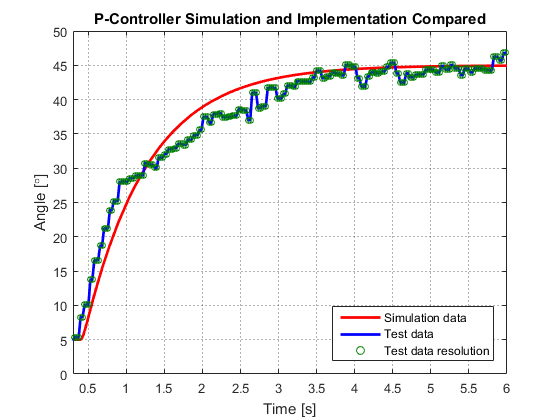
\includegraphics[scale=1]{figures/SteeringAngularTest.png}
 	\caption{Test of the proportional controller, with a start heading on \si{5^{\circ}} and a reference on \si{45^{\circ}}.}
 	\label{fig:AngularTestSim}
\end{figure}\vspace{-5mm}
%
As illustrated in \figref{fig:AngularTestSim}, the system looks similar as the simulation, with the same rise and settling time. The proportional controller is thereby utilized in the system, as it functions inside the area where the system is linear and is stable.

The directional controller is designed, and it is thereby possible to design the the distance controller which is around the directional controller.

\subsection{Distance controller}
A distance controller will now be designed, to complement the angular controller.
As concluded in \secref{sec:SteeringModel}, a deviation from the planned line, will cause the vehicle to drive at a parallel line, next to the planned. The deviation will be calculated from the position provided by the GoT system. As the deviation is a function of the error angle integrated over time it is assumed, that a P controller will be sufficient to handle this function, just as in the Angular controller. The controller will therefore be based on a P controller, and iterated until results are satisfactory. 

As real-world test data is not available, caused by the magnetometer not working in the room with the GoT system installed, the controller will be designed and simulated in Simulink. As a starting point, the proportional gain will be set at 1, and the controller will be designed based on bode plots and step responses.

The proposed controlling scheme can be seen in \figref{SteeringSimulink}

\begin{figure}[H]
\centering
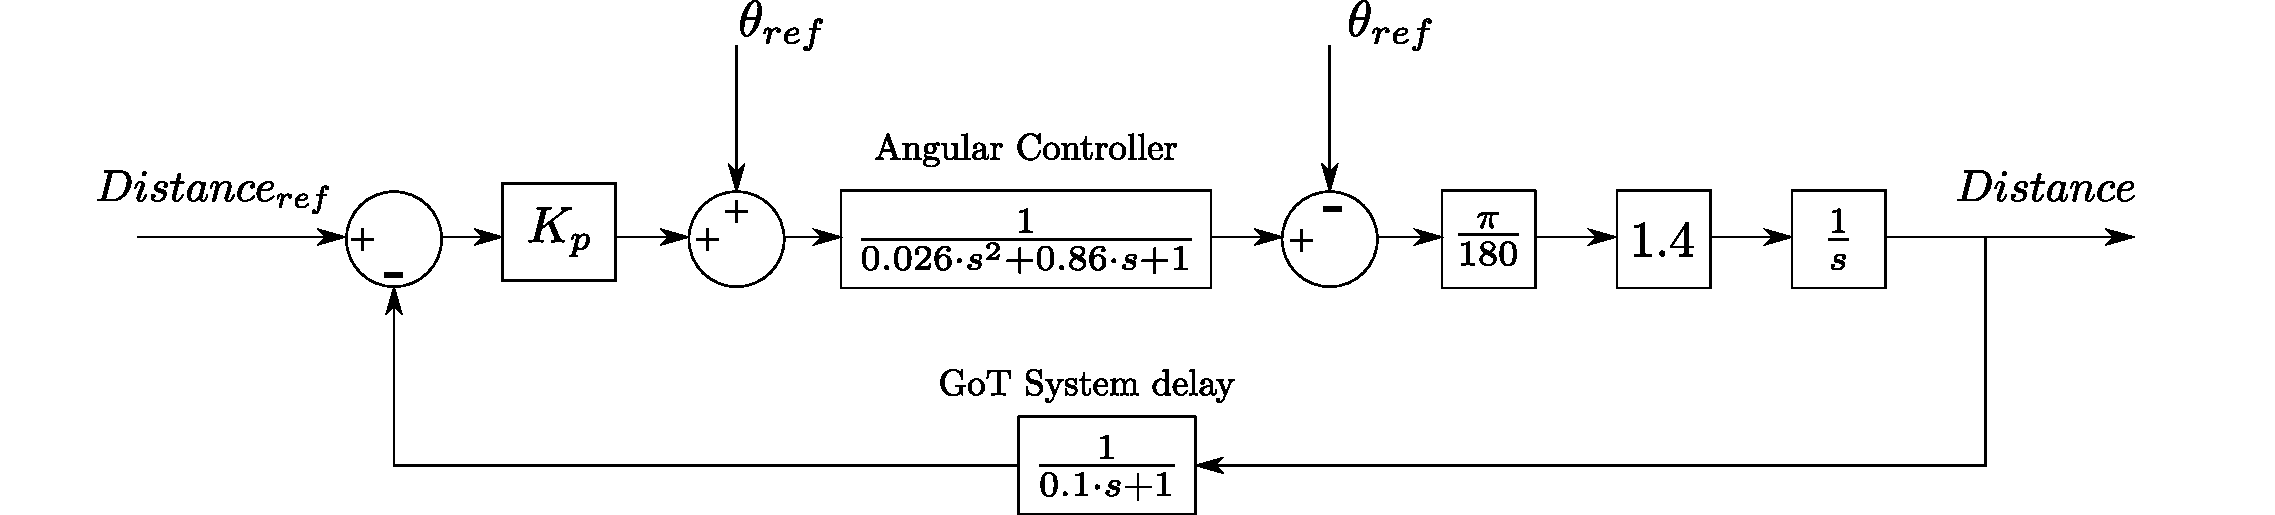
\includegraphics[width=\textwidth]{figures/steeringFullModel.pdf} 
\caption{Initial Distance Controller}
\label{SteeringSimulink}
\end{figure}
As seen in the figure, the Angular Controller is placed in the center of the loop, as this will be responsible for changing the vehicle's angle, to what the distance loop calculates to be necessary. A reference angle, \emph{angleRef} is added to the output of the P controller, representing the angle of the line to follow. To prevent the P controller from over-regulating, and command the system to turn eg. 360 degrees, it is limited by a floor and ceiling of $\pm 90^\circ$. The following three stages (Deg to radians, Velocity and Deviation integrator) are taken directly from the steering model \figref{fig:steeringLineFollowingModel}.

According to \secref{GoTSystem}, the GoT system provides position updates every 100ms. To model this delay, the same approximation as used for the servo delay in \secref{directionalExtention}, will be implemented:
$$\frac{1}{\lambda\cdot\text{s}+1}\leadsto\frac{1}{\SI{0,1}\cdot\text{s}+1}
$$
The input to the loop is the wanted deviation from the line. This should ideally be zero, but is set to 1m in the simulation. This might seem strange, but it is done to force the system to react to an initial error; the error integrator starts at zero when the simulation is started, so an input of zero would imply that the vehicle is not deviating from the planned route, and nothing will happen.
The error could of cause be added at the output, but since the system is assumed linear, a step from 1m to 0m error, should be the same as the opposite.
The resulting step response can be seen in \figref{SimulationSteeringP1}

\begin{figure}[H]
  \centering
 	%Trim margins @:   left        bottom       right       top
 	\adjustbox{ trim = {.15\width} {.30\height} {.15\width} {.30\height}, clip }
  {
    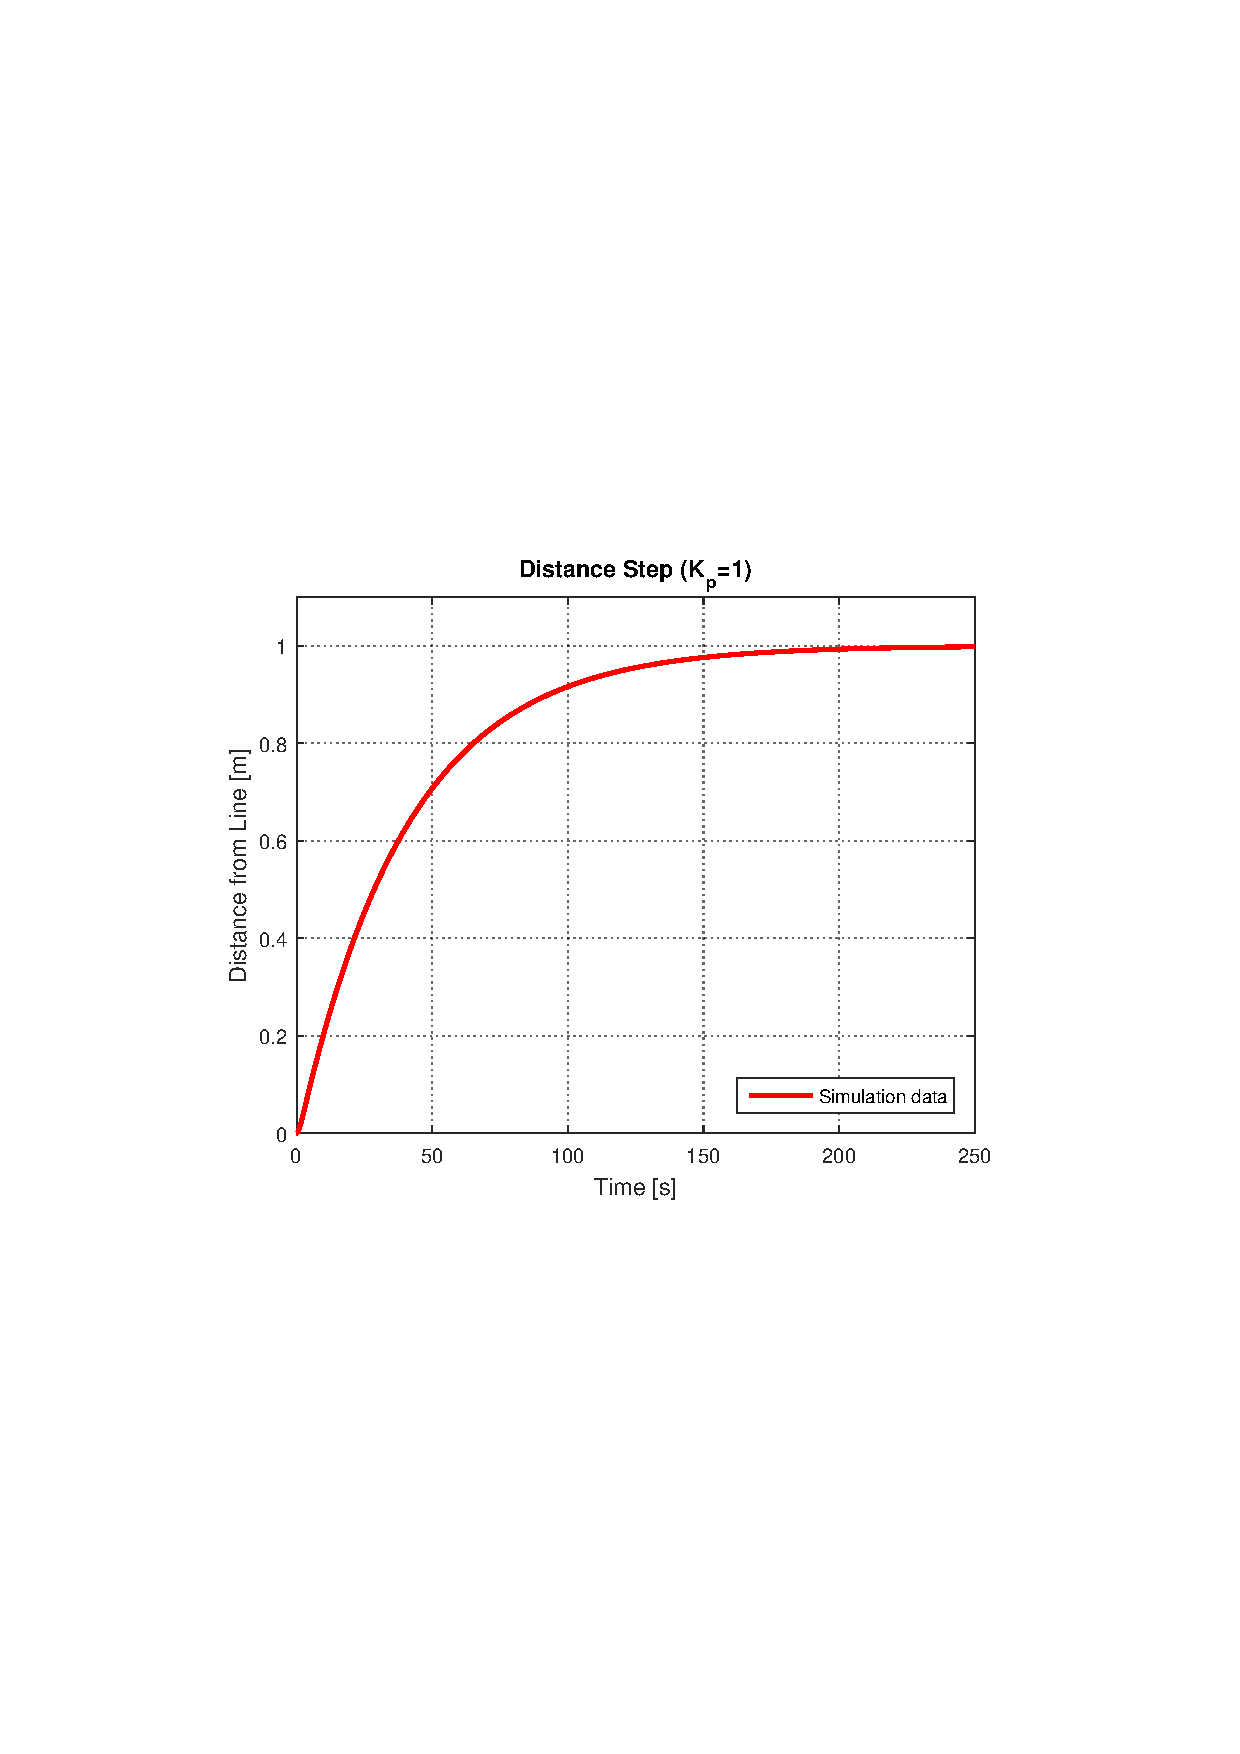
\includegraphics[width=1.4\textwidth]{figures/distanceStep1.pdf}
  }
  \caption{A simulated step-response of the system correcting a 1 meter offset}
  \label{SimulationSteeringP1}
\end{figure}
As seen on the figure, the system takes around 240 seconds, or 4 minutes, to correct the error. This leaves a lot of room for improvements.

Using the Linear Analysis function of Simulink, a Bode plot is made from the open loop system. The resulting plot can be seen in \figref{SimulationSteeringB1}
\begin{figure}[H]
  \centering
 	%Trim margins @:   left        bottom       right       top
 	\adjustbox{ trim = {.15\width} {.30\height} {.15\width} {.30\height}, clip }
  {
    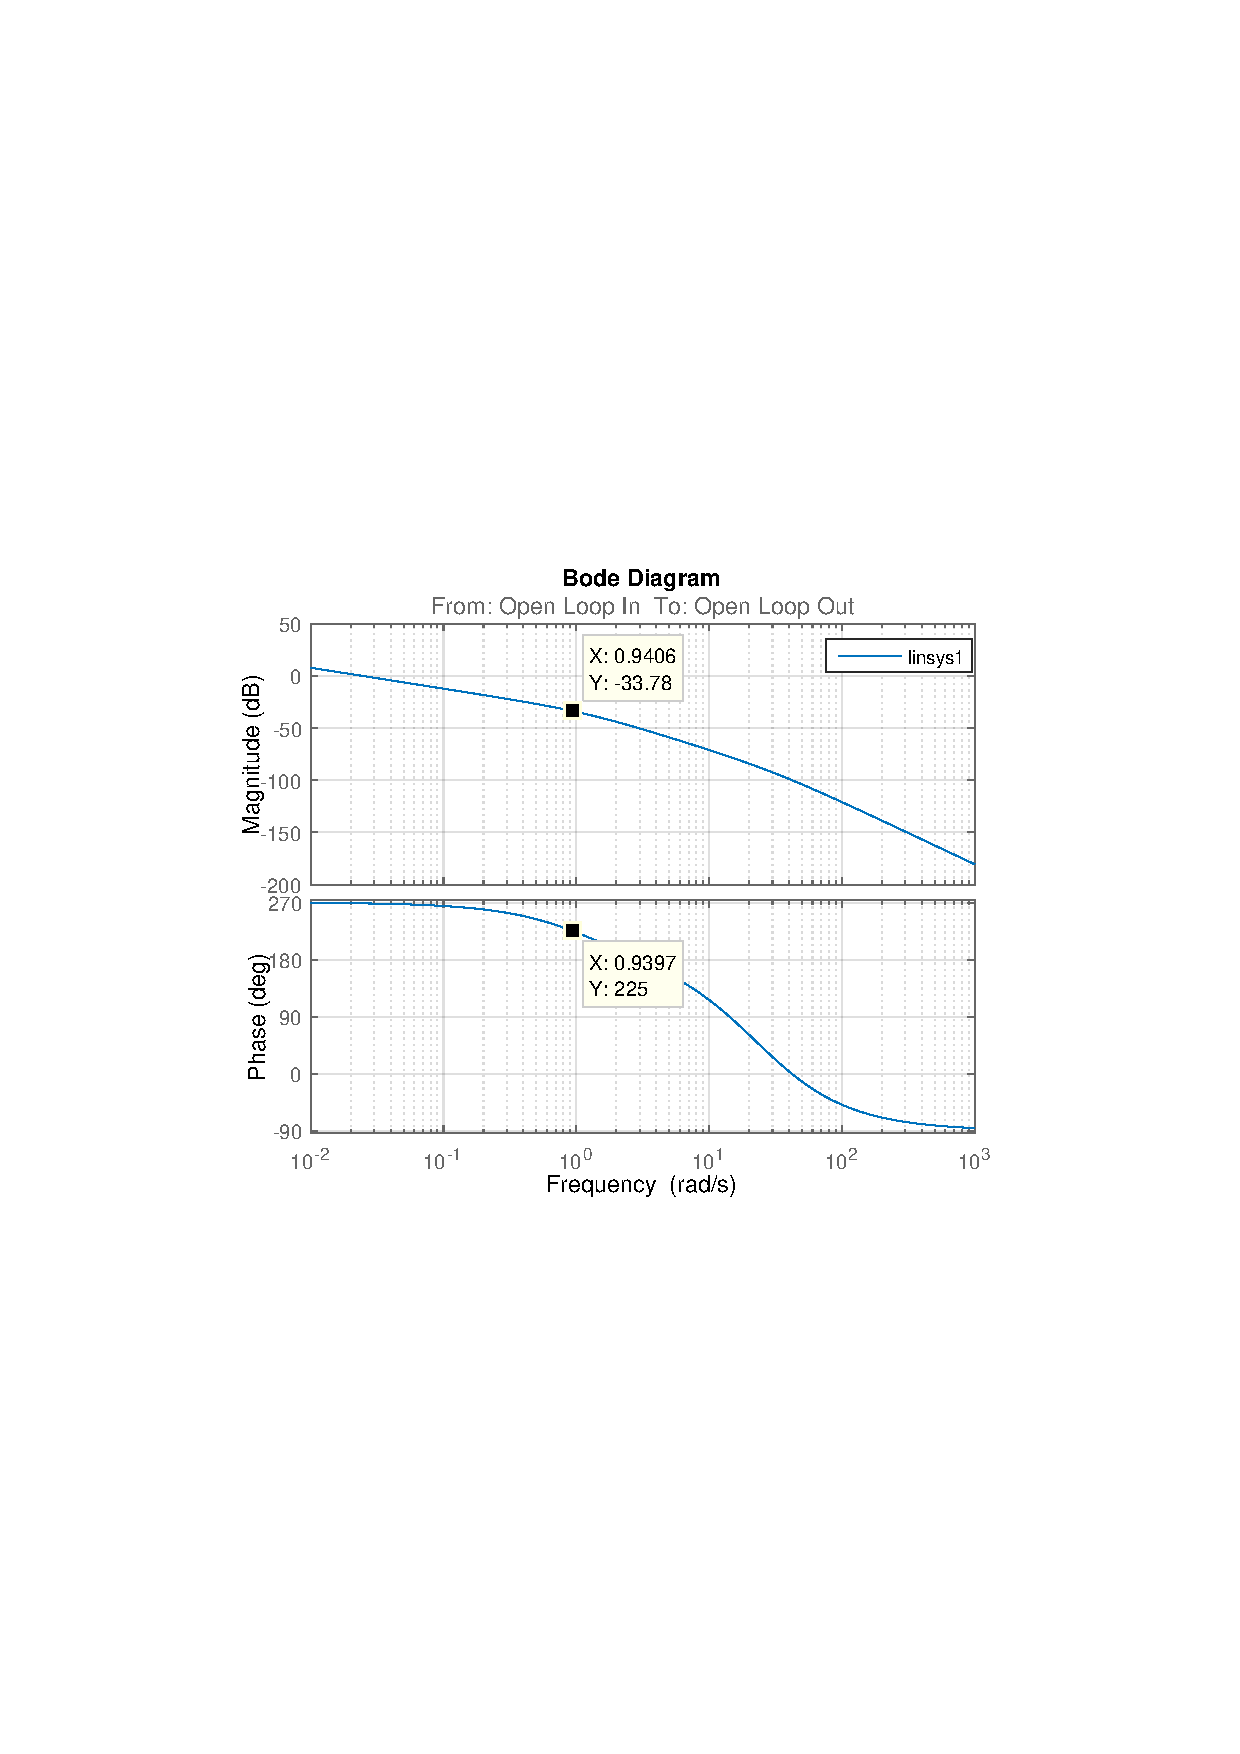
\includegraphics[width=1.4\textwidth]{figures/distanceBode1.pdf}
  }
  \caption{An open loop Bode plot of the system.}
  \label{SimulationSteeringB1}
\end{figure}
To improve the system response, the first thing to be done is to find a better proportional gain than 1. One way to do this, is to optimise for a phase margin of 45 degrees. As seen by the marks on the plots, the gain is \SI{-33,78}dB at the 45 degree point (225-45=180). To get 0 dB gain at this point, the proportional gain will therefore be increased by  \SI{33,78}dB:
$$\text{K}_\text{p}=10^{\frac{\SI{33,78}{}}{20}} = \SI{48,87}{}$$
This value is entered in the simulation, and a new step response is made, see \figref{SimulationSteeringP2}

\begin{figure}[H]
  \centering
 	%Trim margins @:   left        bottom       right       top
 	\adjustbox{ trim = {.15\width} {.30\height} {.15\width} {.30\height}, clip }
  {
    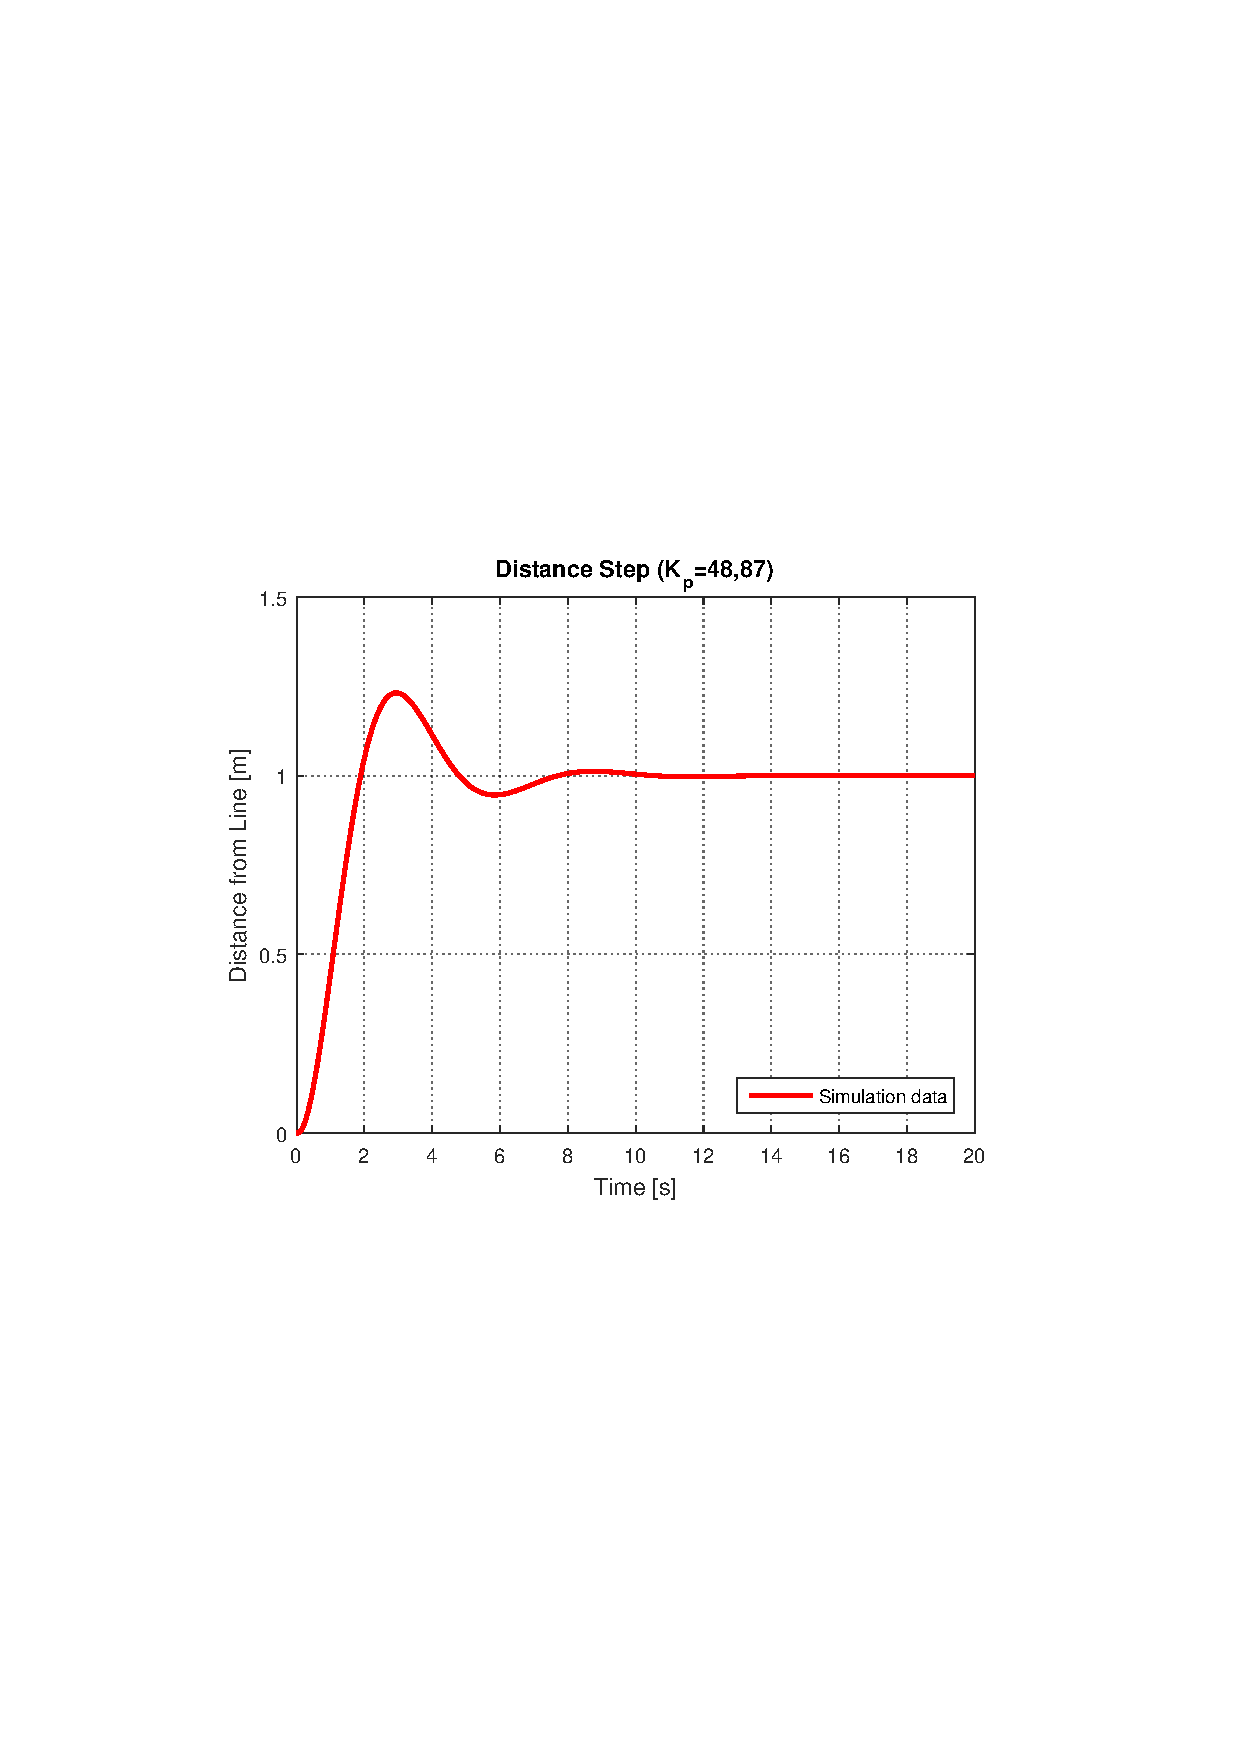
\includegraphics[width=1.4\textwidth]{figures/distanceStep2.pdf}
  }
  \caption{Step response with new $\text{K}_\text{p}$.}
  \label{SimulationSteeringP2}
\end{figure}
As seen in the figure, the response has improved dramatically, and the system reaches the target in approximately 2 seconds. Unfortunately it overshoots and rings, before settling after around 10 seconds. This settling time is a substantial improvement from 4 minutes, but there is still room for further improvements. If the overshoot is removed, the system will reach the target in just 2 seconds.
As seen in the Modeling and Control course on the 5th semester of Electronic and IT at Aalborg University \cite{KMNielsen}, a way to remove an overshoot is to increase the high frequency gain. This can be done by adding a differentiator to the controller, which will then become a PD controller. According to \cite{Franklin}, a PD controller is rarely used in real life, as it is extremely sensitive to noise, and a lead compensator is recommended instead.

A lead compensator adds a zero to the system, which cancels one of the poles in the system. This lowers the phase shift, improving the phase margin, and increases the gain at higher frequencies. At the same time, a pole is added at an even higher frequency, in order to ensure stability.

The sampling period of the loop is limited to 100ms by the GoT system. According to the Nyquist-Shannon sampling theorem, a signal needs to be sampled by at least twice the signal bandwidth. This limits the upper frequency of which the pole in the lead compensator can be placed. To ensure the theorem is fulfilled, the pole is given a time constant of \SI{0,3}{s}. This in turn limits the frequency of the zero - if the zero is placed too close to the pole, they will cancel each other out. On the other hand, it is desired to place the zero as high as possible, in order to not change the low frequency gain, and at the same time to affect the existing poles in the system as much as possible. A compromise must be made, and the zero is given a time constant of 1 second.

A bode plot is made with the lead compensator added to the system, see  \figref{SimulationSteeringB2}. 

\begin{figure}[H]
  \centering
 	%Trim margins @:   left        bottom       right       top
 	\adjustbox{ trim = {.15\width} {.30\height} {.15\width} {.30\height}, clip }
  {
    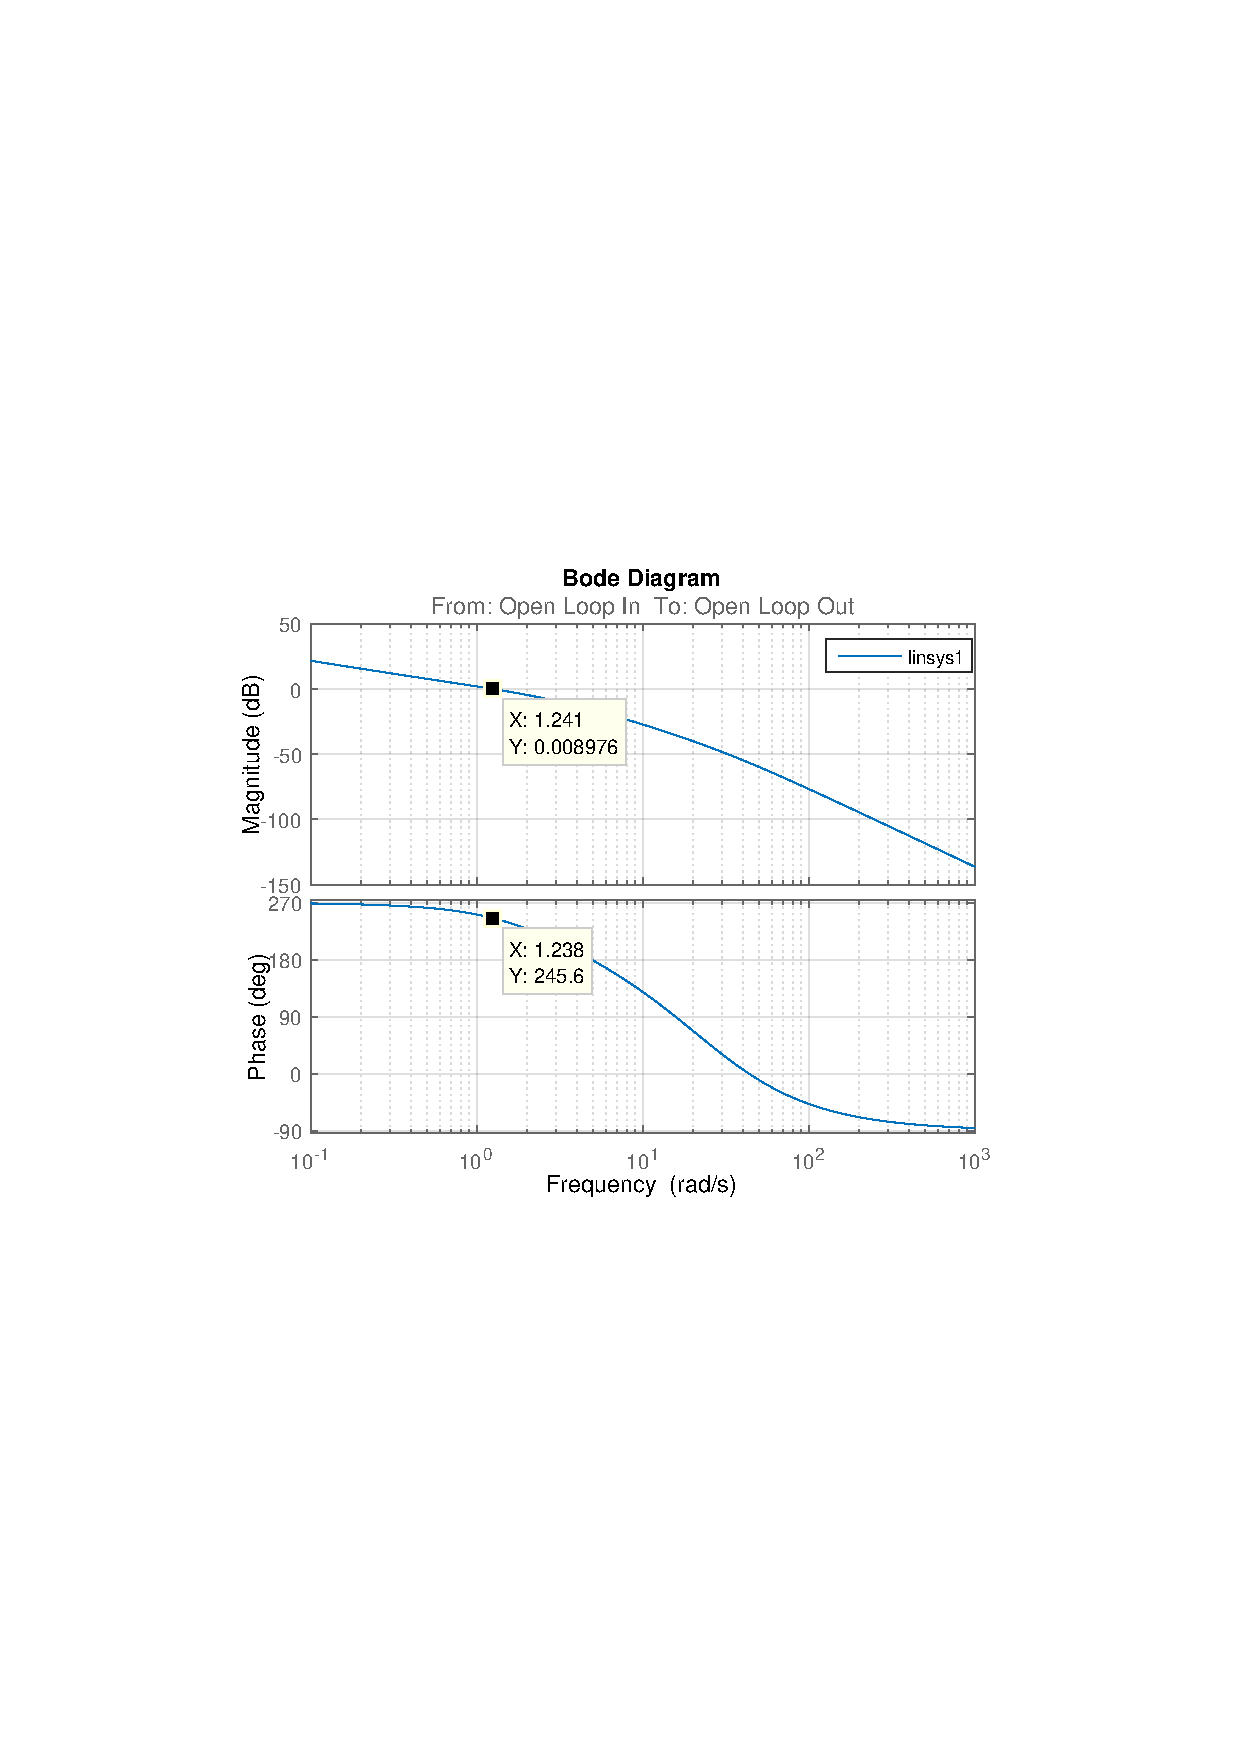
\includegraphics[width=1.4\textwidth]{figures/distanceBode2.pdf}
  }
  \caption{Bodeplot with Lead compensation}
  \label{SimulationSteeringB2}
\end{figure}
The 0 dB frequency has increased from \SI{0,94}{}rad/s to \SI{1,24}{}rad/s, and the phase margin is now: $$\SI{245,6}{}-180=\SI{65,6}{^\circ}$$
As predicted, the lead compensator has increased the gain at higher frequencies and improved the phase margin. This leaves room to increase the proportional gain even further, but before doing this, another step response is made on the system, see \figref{SimulationSteeringP3}.

\begin{figure}[H]
  \centering
 	%Trim margins @:   left        bottom       right       top
 	\adjustbox{ trim = {.15\width} {.30\height} {.15\width} {.30\height}, clip }
  {
    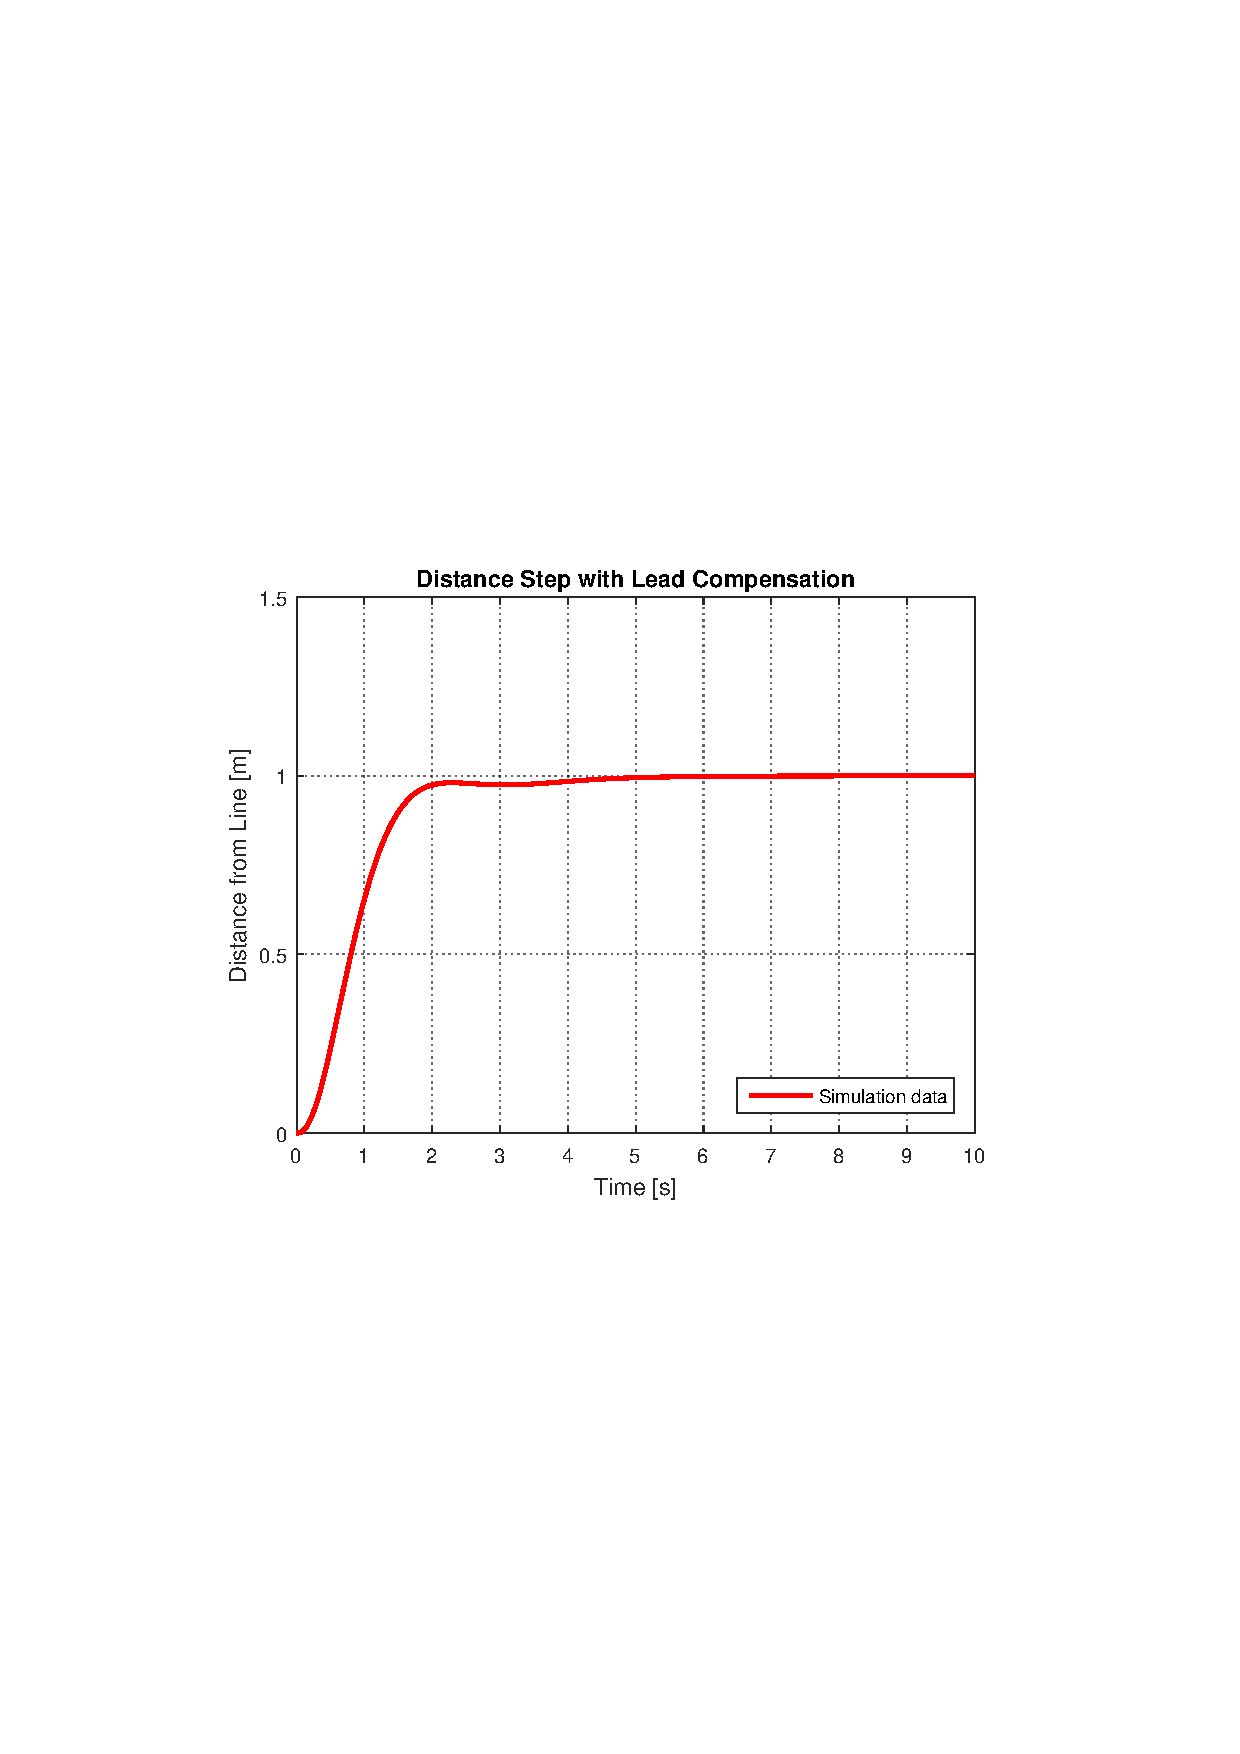
\includegraphics[width=1.4\textwidth]{figures/distanceStep3.pdf}
  }
  \caption{Step response with lead compensation}
  \label{SimulationSteeringP3}
\end{figure}
As seen on the step response, the system reaches the target in approximately two seconds, and the ringing has been reduced to less than \SI{3}{cm}. This is considered acceptable, as it is desirable to keep the increased phase margin. This because the whole loop is based on an approximated model, with no real data to back it up. The extra phase margin will provide a better chance of a stable system in the real world.

\subsection{Route control}
The steering controllers uses information from the route, that it have to follow. The route is made up by a number of points in the coordinate system from the GOT system, which there is drawn lines between , shown on \figref{fig:RCfig1}.

\begin{figure}[H]
 	\centering
 	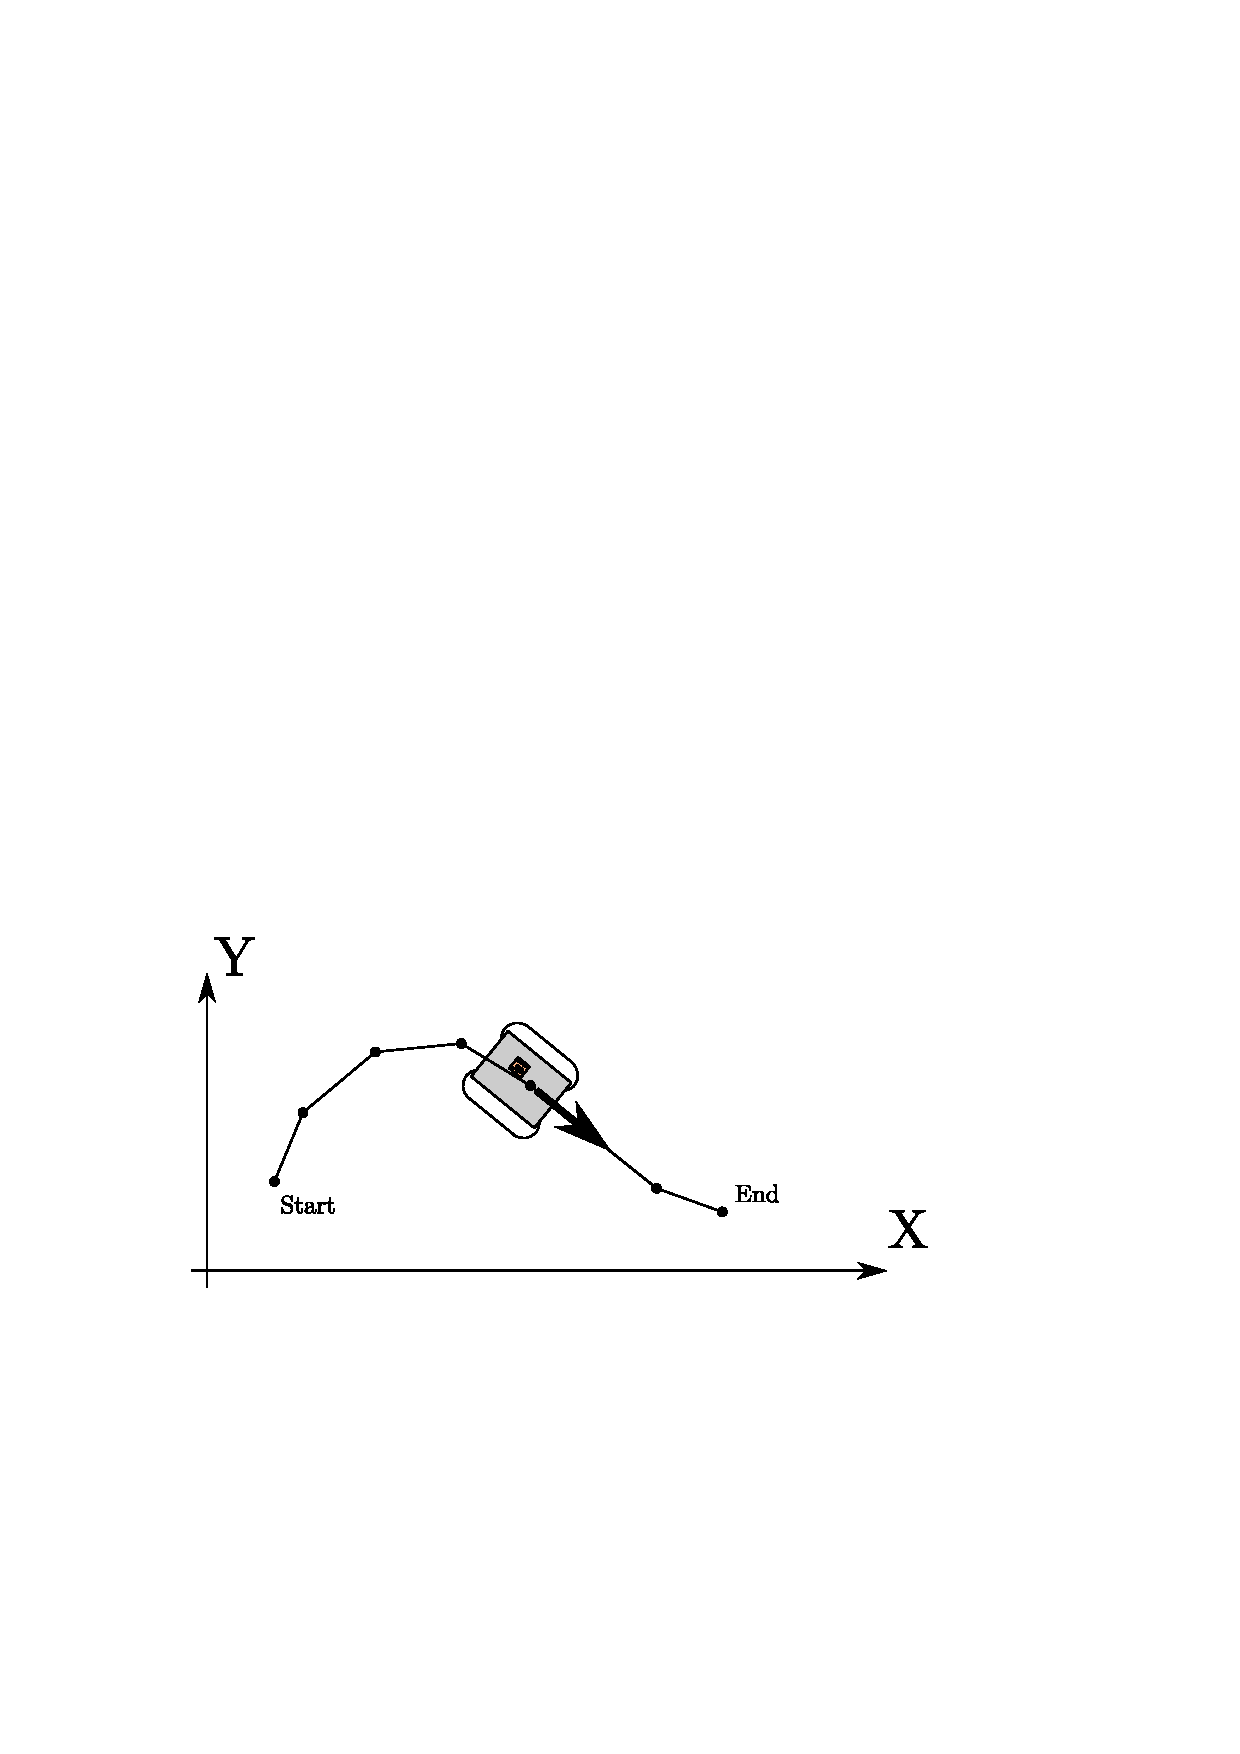
\includegraphics[scale=0.7]{figures/stepsGoT}
 	\caption{An example of a route, where the contains 7 points, which the vehicle have to follow.}
 	\label{fig:RCfig1}
\end{figure}

\subsubsection{Angle}
The angular controller needs the angle of the route line, that is added to the output from the distance controller, to be the reference angle for the controller. The lines is made by connection the points the route and therefore only the start and end point of each line is known. To calculate the angle of the line, compared to the coordinate system of the GOT system, \eqref{eq:RCeq1} is used.

\begin{flalign}
  \eq{\theta_{line}}{tan^{-1}(\frac{Y_{end}-Y_{start}}{X_{end}-X_{start}}) \cdot \frac{180}{\pi}}\unit{\si{^\circ}}\label{eq:RCeq1}
\end{flalign}

As the output from the inverse tangent is in $rad \cdot s^{-1}$, it is multiple by $\frac{180}{\pi}$ to convert it to degrees. With this equation, zero degrees will be in the direction of the positive x axis and it will go counter clockwise for positive angles and clockwise for negative angles. This give a range from \si{-180^\circ} to \si{180^\circ}, which also is the output from the magnetometer. If it is compared, the angle from the coordinate system for the GOT system, is not equal to the angle, that comes from the magnetometer. The reason for this is that the positive x axis is not going in the same direction as north. Therefore there is needed a offset angle, that rotates the coordinate system, so zero degrees for the coordinate system and the magnetometer is the same direction.

There will be a mathematical problem, if the X coordinates is the same for both points, as there will be divided by zero. If the X values is the same, the angle will be either 90 degrees, if going toward positive y axis, or -90 degrees, if going the opposite way. As the different can be seen on the difference in the Y value, the function will return the right numbers, even if is should not be mathematically possible to calculate it.

As the magnetometer do not work in the GOT room, this offset angle cannot be measured and therefore can the right angle of the line not be calculated and used at indoor test.

\subsubsection{Distance}
The distance controller needs the distance from the vehicle to the route line, as it use this value as a error value. The distance can be calculated with \eqref{eq:RCeq2}.

\begin{flalign}
  \eq{Distance}{\frac{(a \cdot X_{now}) + (b \cdot Y_{now}) + c)  }{\sqrt{a^2 + b^2}}}\unit{m}\label{eq:RCeq2}
\end{flalign}
\\
\begin{figure}[H]
 	\centering
 	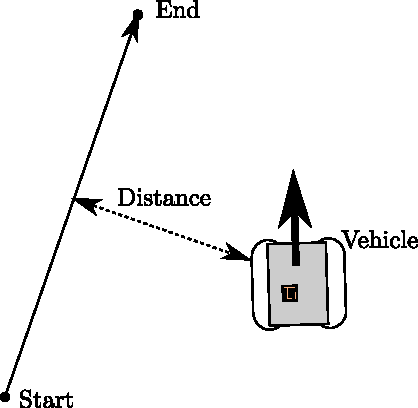
\includegraphics[scale=0.8]{figures/DistanceOutLoop}
 	\caption{Illustration of the distance, that is calculated. The line, that comes from the shortest distance, is orthogonal on the route line.}
 	\label{fig:RCfig2}
\end{figure}

\eqref{eq:RCeq2} is a standard vector equation to calculate the shortest distance from a point to a line (See \figref{RCfig2}). The a, b and c values can be calculated from the start and end point, by using \eqref{eq:RCeq3}, \eqref{eq:RCeq4} and \eqref{eq:RCeq5}.

\begin{flalign}
  \eq{a}{Y_{end} - Y_{start}}\unit{m}\label{eq:RCeq3} \\
  \eq{b}{X_{start} - X_{end}}\unit{m}\label{eq:RCeq4} \\
  \eq{c}{X_{end} \cdot Y_{start} - Y_{end} \cdot X_{start}}\unit{m}\label{eq:RCeq5}
\end{flalign}

From \eqref{eq:RCeq2}, the distance is calculated. If the distance is negative, the vehicle is on the left side of the line and on the right side, when the distance i positive. With this equation and the measured coordinate from the GoT system, the distance the vehicle is away from the line is known and can be used as a error in the distance controller.

\subsubsection{New line}
When the vehicle reach the end point of a line on the route, a new line is used to calculate the angle and distance. The new line's start point will be the last line's end point, so the route lines is connected. Then the next end point is set and the angle can be calculated and the distance measured.

As the GOT system have a precision down to 1 mm, the coordinates too have a precision of 1 mm \todo{Ref to GOT}. The vehicle will not hit the end point with this precision, as the GOT system only give a measurement each 100 ms , and if the vehicle travels with 1,4 $m \cdot s^{-1}$ \todo{ref to velocity controller}, it will travel 140 mm for each measurement, which make the chance for hitting the end point exactly, small. Therefore is the area, which indicates the end of the route line, made bigger. The size out should be around twice as big as the distance, that the vehicle travels between each measurement. With this size, there will always be two measurement in the circle, so the even if one of the measurements is not good, there will be another one. This will give a circle with a radius of 28 cm

\todo{Insert perfect tail, please}
